
\documentclass[11pt]{article}
 
\usepackage[margin=1in]{geometry} 
\usepackage{amsmath,amsthm,amssymb}
\usepackage{graphicx} 
\usepackage{blkarray}
\usepackage{amsmath}




\newcommand{\N}{\mathbb{N}}
\newcommand{\Z}{\mathbb{Z}}
 
\newenvironment{problem}[2][Problem]{\begin{trivlist}
\item[\hskip \labelsep {\bfseries #1}\hskip \labelsep {\bfseries #2.}]}{\end{trivlist}}
\newenvironment{lemma}[2][Lemma]{\begin{trivlist}
\item[\hskip \labelsep {\bfseries #1}\hskip \labelsep {\bfseries #2.}]}{\end{trivlist}}
\newenvironment{exercise}[2][Exercise]{\begin{trivlist}
\item[\hskip \labelsep {\bfseries #1}\hskip \labelsep {\bfseries #2.}]}{\end{trivlist}}

\newenvironment{question}[2][Question]{\begin{trivlist}
\item[\hskip \labelsep {\bfseries #1}\hskip \labelsep {\bfseries #2.}]}{\end{trivlist}}
\newenvironment{corollary}[2][Corollary]{\begin{trivlist}
\item[\hskip \labelsep {\bfseries #1}\hskip \labelsep {\bfseries #2.}]}{\end{trivlist}}

\usepackage{indentfirst}
\linespread{1.2}     % 调整间距
\setlength{\parindent}{0pt}

\begin{document}

 
% --------------------------------------------------------------
%                         Start here
% --------------------------------------------------------------
 
\title{Homework 11 DS-GA 1002 }%replace X with the appropriate number
\author{Yuhao Zhao\\ %replace with your name
Yz3085} %if necessary, replace with your course title
\maketitle

\begin{problem}{1}
\end{problem}
a) $f := \sum_{i = 1}^{n} a_if_i$ and $f_i‘s$ are convex functions. \\
for $\forall x,y \in R $ and $\theta \in [0,1]$, $\theta f(x)+ (1-\theta)f(y) =\theta \sum_{i = 1}^{n} a_if_i(x) +(1-\theta) \sum_{i = 1}^{n} a_if_i(y) \\ = \sum_{i = 1}^{n}  a_i(\theta f_i(x) + (1- \theta)f_i(y))$ \\ Since $f_i‘s$ are convex, $\theta f_i(x) + (1- \theta)f_i(y) \geq f_i(\theta x + (1-\theta)y)$\\
if $a_i's$ are non-negative, $a_i(\theta f_i(x) + (1- \theta)f_i(y)) \geq a_i f_i(\theta x + (1-\theta)y)$\\
Therefore, $RHS \geq \sum_{i = 1}^{n} a_i f_i(\theta x + (1-\theta)y) = f(\theta x + (1-\theta)y)$\\
Thus, f is convex.\\

b) $g = \max\limits_{1\leq i \leq m} f_i(x)$\\
for $\forall x,y \in R $ and $\theta \in [0,1]$, $\theta g(x) + (1- \theta)g(y) = \max \theta f_i(x) + \max  (1 - \theta) f_i(y)$\\
We claim that $\sup (f+ g) \leq \sup (g) +\sup (f)$\\
since $f\leq \sup  f, g\leq \sup  g, f+g \leq \sup (f) +\sup (g)\\\sup (f + g) \leq \sup (\sup (f)+\sup (g)) = \sup (f) +\sup (g))$\\
Therefore, $\max \theta f_i(x) + \max  (1 - \theta) f_i(y) \geq \max \theta f_i(x)  +   (1 - \theta) f_i(y) = g(\theta x+ (1 - \theta)y) \\$
Thus, g is convex\\

c) $h: = \prod_{i =1}^{m} f_i$\\
counterexample: $f_1 = 1-x$, $f_2 = 1+x$\\
$f_1,f_2 $ are convex since $f''_1 \equiv 0 , f''_2 \equiv 0.$\\
$ h= f_1f_2 = 1- x^2$, $h'' = -2 <0$\\
h is not convex.\\

\begin{problem}{2}
\end{problem}
Code:
\begin{verbatim}
def derivative_descent(x_ini, f, der_f, step, eps):
        if abs(der_f(x_ini)) > eps:
        return [x_ini] + derivative_descent(x_ini-step*der_f(x_ini),f,der_f,step,eps)
        else:
        return [x_ini]


def newton_method(x_ini, f, der_f, der2_f, eps):
        if abs(der_f(x_ini)) > eps:
        return [x_ini] + newton_method(x_ini- (der_f(x_ini)/der2_f(x_ini))
                                       ,f, der_f, der2_f, eps)
        else:
        return [x_ini]  
		
def quadratic_approx(x, point, f, df, d2f):
        return f(point)+df(point)*(x- point) +0.5*d2f(point)*(x-point)**2
\end{verbatim}


\begin{problem}{3}
\end{problem}
a) The projection of a vector $x \in R^n$ on the positive orthant $R_+^n$ is :\\
1. x, if x $\in R_+^n$\\
2. The closest point $x^* \in R_+^n$ that minimize the distance between $x $ and $ x^*$ which is: \\
$\min\limits_{x^* \in R_+^n} ||x - x^*|| =\min\limits_{x^* \in R_+^n} \sum (x_i - x_i^*)^2$\\
The solution is equivalent to minimize the difference in each coordinates. The projection is indeed $x^*_i = I(x_i \geq 0) x_i$ \\

b) The projection of a vector $x \in R^n$ on the unit $\l_2 $ ball $B_{\l_2}$ is :\\ 
1. x, if x $\in  B_{\l_2}$\\
2. The closest point $x^* \in B_{\l_2}$ that minimize the distance between $x $ and $ x^*$ \\
We claim that $x^* \in span(x)$:\\
If not, let the projection $x^* \notin span(x)$\\
by triangular inequality  $||x^*|| + ||x- x^*|| \geq ||x||$, we know that $||x^*|| \leq 1$\\
we can find a vector $\tilde{x} \in span(x)$ and $||\tilde{x}|| = ||x^*||, \tilde{x} \in B_{\l_2}$\\
Then $||x - \tilde{x}|| = ||x|| - ||\tilde{x}|| \leq ||x^*|| + ||x - x^*|| - ||\tilde{x}|| = ||x - x^*|| $\\
Then $x^* $ is not he closet vector to x in $B_{\l_2}$ which is a contradiction \\


We claim also that $x^* \in \partial B_{\l_2}$(Boundary of the set):\\
if not, let the projection $\tilde{x}\in  B_{\l_2}^\circ$(Interior of the set)  and $\tilde{x} \in span(x)$\\
$||\tilde{x}|| \leq 1$, we can find $x^* \in span(x),$ and $||x^*|| = 1$\\
$||x-x^*|| \leq ||x - \tilde{x}||$ This is a contradiction.\\
Therefore, solution is $\frac{x}{||x||_2}$ if $x \notin B_{\l_2}$ and x if $x \in B_{\l_2}$\\

c) Code:\\
\begin{verbatim}
def projected_gradient_descent(x_ini, f, grad, step, eps, proj, n_iter):
    curr = proj(x_ini)
    res = np.matrix(curr)
    n = 0
    if np.dot(grad(curr),grad(curr)) <= eps:
           return res 
    else: 
           while  np.dot(grad(curr),grad(curr)) > eps:
           curr = proj(curr - step*grad(curr))
           res = np.vstack((res,curr))
           n += 1
           if n==10:
                return res

def projection_positive(x):
    dim = len(x)
    return np.array((x>=0)* x)

def projection_l2(x):
    norm = np.sqrt(np.dot(x,x))
    return x/norm if norm>1 else x
\end{verbatim}

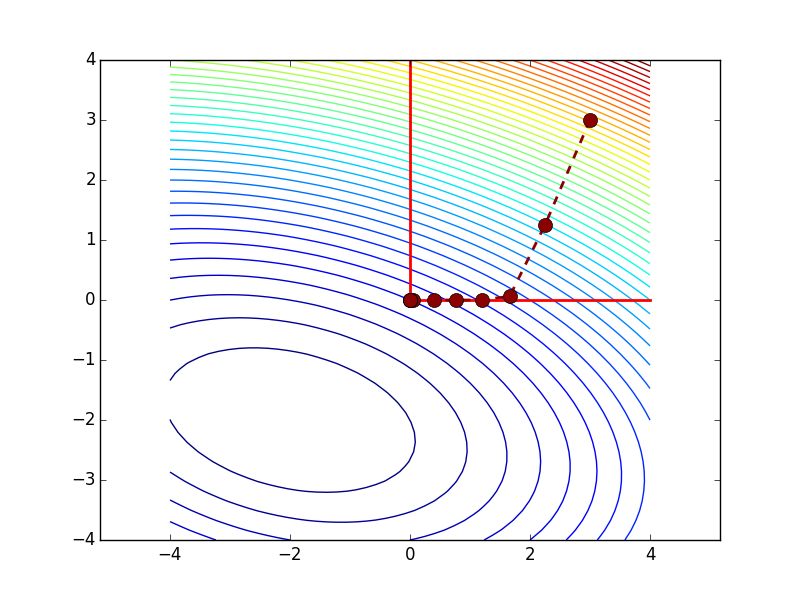
\includegraphics[width = 4.1in]{3-1}\\
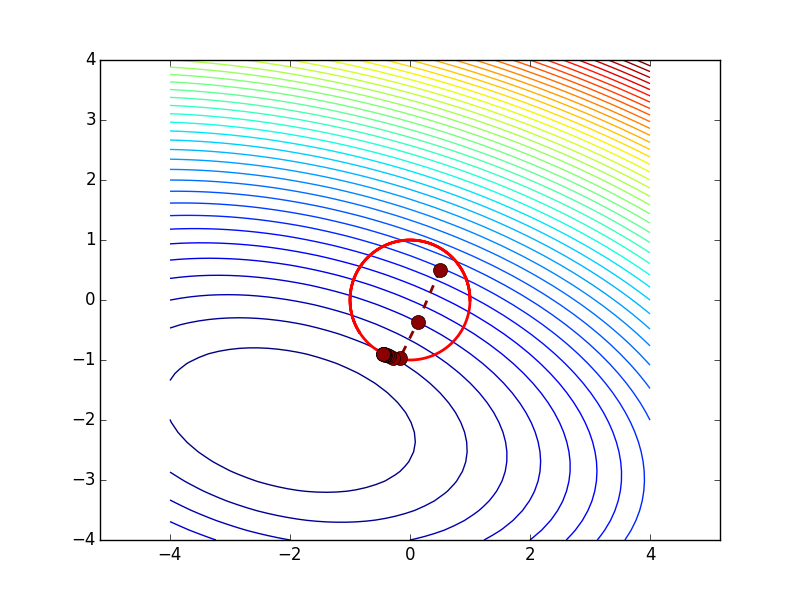
\includegraphics[width = 4.1in]{3-2}\\

d) The projection positive will converge to (0,0) since it's the closet solution in the positive orthant to the global solution (it lies on the smallest contour line). The projection l2 will converge to $(-\frac{\sqrt{2}}{2},-\frac{\sqrt{2}}{2})$






\end{document}